\section{МЕТОДИКА РАСЧЁТА И ПРОГРАММНАЯ РЕАЛИЗАЦИЯ} %заменить



\subsection{Общие алгоритмы и структуры}

В данном подразделе перечислены основные алгоритмы и структуры, которые использовались в остальных модулях. Сюда вошли алгоритмы LU-разложения матрицы, QR алгоритм нахождения собственных чисел матрицы, алгоритмы дифференцирования с разным порядком точности и так далее. Для работы с таблицами Бутчера и алгоритмами решения СНУ был реализован собственный класс матрицы с базовой матричной алгеброй. Для комфортной работы с конечно-разностной схемой были написаны структуры для перевода величин из физических в профильные, функции для компактного вычисления больших множителей и так далее.

\textit{LU алгоритм}

LU-разложение матрицы \cite{Article1} $A$ представляет собой разложение матрицы $A$ в произведение нижней и верхней треугольных матриц, т.е. $A = LU$, где $L$ ~--- нижняя треугольная матрица на диагонали которой стоят единицы, $U$ ~--- верхняя треугольная матрица. LU–разложение может быть использовано при решении систем линейных алгебраических уравнений вида $Ax = b$. Полученное LU-разложение может быть так же использовано для вычисления определителя матрицы по формуле.

\begin{equation}
    det(A) = det(L)det(U) = (\prod\limits_{i = 1}^nL_{ii})(\prod\limits_{i = 1}^nU_{ii}) = \prod\limits_{i = 1}^nU_{ii},
    \label{eq:Det}
\end{equation}

где $n$ ~--- размер квадратной матрицы.

Для нахожения обратной матрицы из задачи $AX = E$, где $A$ ~--- исходная матрица, $X$ ~--- обратная матрица, $E$ ~--- единичная
матрица, составляется $n$ систем уравнений:
\begin{equation}
    \begin{gathered}
        AX_i = e_i,  i = 1, ..., n,
    \end{gathered}
    \label{eq:Reverse}
\end{equation}

где $X_i$ ~--- вектор-столбец обратной матрицы с индексом $i$, $e_i$ ~--- вектор-столбец единичной матрицы с индексом $i$.

Нахождение обратной матрицы сводится к решению $n$ уравнений с одной матрицей и разными правыми частями.

\textit{Метод Гаусса}

Метод Гаусса ~--— это прямой численный метод решения систем линейных алгебраических уравнений (СЛАУ) вида:

\begin{equation}
\begin{split}
Ax &= b,
\end{split}
\label{eq_gauss}
\end{equation}
где $A$ ~--- матрица коэффициентов размера $n \times n$, $x$ ~--- вектор неизвестных, $b$ ~--- вектор правых частей.

Цель метода: преобразовать исходную систему к треугольному виду (прямой ход), а затем найти неизвестные обратной подстановкой (обратный ход).

При сравнении производительности методов Гаусса с выбором главного элемента и LU-разложения для решения системы вида ~\ref{eq_gauss}, было установлено, что метод Гаусса обладает лучшей устойчивостью и скоростью решения. LU-разложение матрицы используется для нахождения обратной матрицы при вычислении Якобиана в части решения химической кинетики.

\textit{Дифференцирование}

Для численного дифференцирования была разработана функция, получающая  получающая в качестве аргументов функцию для дифференцирования,
точку, в которой необходимо продифференцировать функцию и схему дифференцирования:

\begin{equation}
    y' = \frac{a_1y_{i-n+1} + a_2y_{i-n+2} + ... + a_{2n-1}y_{i+n-1}}{ch^p}
    \label{eq:DiffCommon}
\end{equation}

где $n$ ~--- количество точек аппроксимации.

При таком представлении все схемы можно реализовать при помощи одномерного массива коэффициентов.

$$
[a_1, a_2, ..., a_{2n - 1}, c, p]
$$

где $a_i$ ~--- коэффициенты для точек, $c$ ~--- коэффициент перед шагом в знаменателе, $p$ ~--- степень шага. Такой подход позволяет
быстро дополнять текущий набор схем новыми. Помимо этого избегается дублирование одинакого кода.
Так, например, вторая 4-х точечная схема 

\begin{equation}
    y_i' = \frac{-11y_{i} + 18y_{i+1} - 9y_{i+2} + 2y_{i+3}}{6h}
    \label{eq:Diff1-4}
\end{equation}

может быть представлена в следующем виде:

$$
[0, 0, 0, -11, 18, -9, 2, 6, 1]
$$

\textit{Общие упрощения и оптимизации по коду}

Для просчёта прогоночных коэффициентов трёхдиагональной матрицы требуется достаточно много слагаемых, содержащих сразу несколько множителей. Для улучшения написания кода было реализовано несколько вспомогательных лямбда-функций. Рисунки ~\ref{src:lamda_optimization_1}, ~\ref{src:lamda_optimization_2} показывает листинг, содержащий код таких функций.

\begin{figure}
\begin{lstlisting}[language=C++]
    auto comp = [&] (const std::vector<uint64_t> &numerator, const std::vector<uint64_t> &denominator, uint64_t n, uint64_t m) -> double {
        double ans = 1.0;
        for (uint64_t i : numerator) {
            ans *= i == Y ? std::pow(f[i](n, m), nu) : f[i](n, m);
        }
        for (uint64_t i : denominator) {
            ans /= i == Y ? std::pow(f[i](n, m), nu) : f[i](n, m);
        }
        return ans;
    };
    auto compAlpha = [&] (const std::vector<uint64_t> &numerator, const std::vector<uint64_t> &denominator, uint64_t n, uint64_t m) -> double {
        return (1.0 - alpha) * comp(numerator, denominator, n - 1, m) + alpha * comp(numerator, denominator, n, m);
    };
    auto compd = [&] (char firstDiff, const std::vector<uint64_t> &num1, const std::vector<uint64_t> &denum1, uint64_t n, uint64_t m) -> double {
        double ans = 0.0;
        if (firstDiff == 'x') {
            ans = 1.0 / (2 * L) * (comp(num1, denum1, n + 1, m) - comp(num1, denum1, n - 1, m));
        }
        if (firstDiff == 'y') {
            if (m == 0) {
                ans = 1.0 / H * (comp(num1, denum1, n, m + 1) - comp(num1, denum1, n, m));
            } else if (m == f[0].size().m - 1) {
                ans = 1.0 / H * (comp(num1, denum1, n, m) - comp(num1, denum1, n, m - 1));
            } else {
                ans = 1.0 / (2 * H) * (comp(num1, denum1, n, m + 1) - comp(num1, denum1, n, m - 1));
            }
        }
        return ans;
    };
\end{lstlisting}
\caption{Код вспомогательных функций}
\label{src:lamda_optimization_1}
\end{figure}

\begin{figure}
\begin{lstlisting}[language=C++]
    auto compdd = [&] (char firstDiff, const std::vector<uint64_t> &num1, const std::vector<uint64_t> &denum1, char secondDiff, const std::vector<uint64_t> &num2, const std::vector<uint64_t> &denum2, uint64_t n, uint64_t m) -> double {
        double ans = 0.0;
        if (firstDiff == 'x' && secondDiff == 'x') {
            ans = 1.0 / L * (comp(num1, denum1, n + 1, m) * (comp(num2, denum2, n + 1, m) - comp(num2, denum2, n, m)) / L - comp(num1, denum1, n - 1, m) * (comp(num2, denum2, n, m) - comp(num2, denum2, n - 1, m)) / L);
        }
        if (firstDiff == 'x' && secondDiff == 'y') {
            ans = 1.0 / (2 * L) * (comp(num1, denum1, n + 1, m) * (comp(num2, denum2, n + 1, m + 1) - comp(num2, denum2, n + 1, m - 1)) / (2 * H) - comp(num1, denum1, n - 1, m) * (comp(num2, denum2, n - 1, m + 1) - comp(num2, denum2, n - 1, m - 1)) / (2 * H));
        }
        if (firstDiff == 'y' && secondDiff == 'x') {
            ans = 1.0 / (2 * H) * (comp(num1, denum1, n, m + 1) * (comp(num2, denum2, n + 1, m + 1) - comp(num2, denum2, n - 1, m + 1)) / (2 * L) - comp(num1, denum1, n, m - 1) * (comp(num2, denum2, n + 1, m - 1) - comp(num2, denum2, n - 1, m - 1)) / (2 * L));
        }
        if (firstDiff == 'y' && secondDiff == 'y') {
            ans = 1.0 / H * (comp(num1, denum1, n, m + 1) * (comp(num2, denum2, n, m + 1) - comp(num2, denum2, n, m)) / H - comp(num1, denum1, n, m - 1) * (comp(num2, denum2, n, m) - comp(num2, denum2, n, m - 1)) / H);
        }
        return ans;
    };
\end{lstlisting}
\caption{Код вспомогательных функций}
\label{src:lamda_optimization_2}
\end{figure}

\subsection{Графический пользовательский интерфейс}

Для ввода задачи была реализована специальная форма с использованием библиотеки \textit{OpenGL}. Её внешний вид представлен на рисунке \ref{fig:forma1}.

Ввод начальных условий происходит посредством чтения их из файла, форму можно использовать для выбора необходимого файла с набором данных, отображения результатов вычисления, проигрывания анимации, а так же анализа точности, производительности и изменению значений переменных на протяжении всего расчёта. По окончанию вычислений, все результаты сохраняются в отдельный файл, поэтому решать тестовые наборы достаточно один раз (если не планируется их дальнейшее изменение).

\begin{figure}
    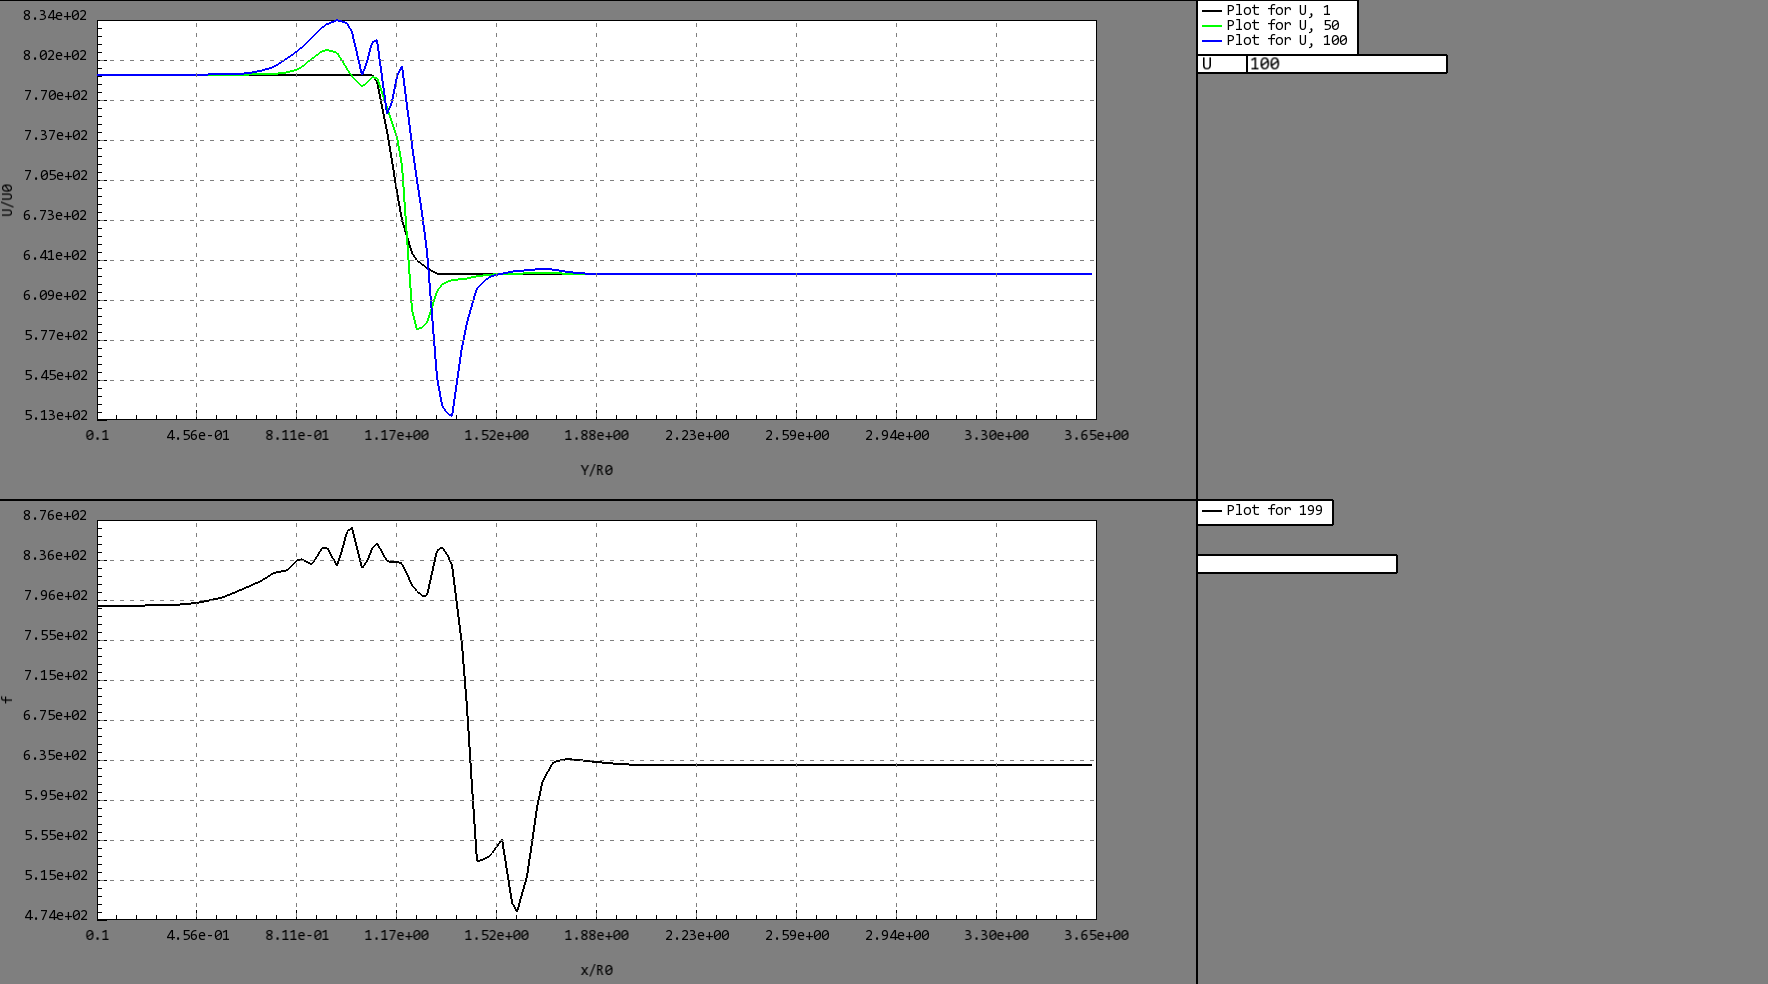
\includegraphics[width=15cm]{2-04-new_form}
    \caption{Вид интерфейса для ввода анализа решения}
    \label{fig:forma1}
\end{figure}

После ввода задачи и экспериментальных данных (при наличии), начальных условий и границ интегрирования требуется выбрать метод решения.

\subsection{Парсер химичесских уравнений}

Химические уравнения обычно записываются в виде

\begin{equation}
    Sub_1 + Sub_2 \Longleftrightarrow Sub_3 + Sub4,
    \label{eq:Chemic}
\end{equation}

где $Sub_i$ ~--- некоторые вещества. Помимо формул, для моделирования реакций нужно знать термодинамические свойства веществ и Аррениусовские константы скоростей для каждой реакции~\cite{book3}.

На основе этих данных формируется СДУ, порядок которой равен числу веществ, участвующих в реакциях \cite{Article5}. Подробнее про это расписано в предыдущем разделе.

\subsection{Реализация методов решения СДУ}

Как уже говорилось выше, все методы семейства Рунге-Кутты можно представить в виде таблиц Бутчера \cite{cite_1_3}. В связи с этим появилась идея реализовать алгоритм, принимающий в качестве аргументов задачу и таблицу Бутчера и возвращающий решение в виде таблицы с координатами. Благодаря этому алгоритму добавлять новые методы не вызывает никаких сложностей. Используемые методы перечислены на рисунке \ref{fig:SolveMethods}. Всего в данной работе используется 62 схемы со 2 по 6 порядок точности. Для решения зачач горения используются явная схема Рунге-Кутты и неявная схема Гаусса. Обе схемы 6-го порядка точности.

\begin{figure}
    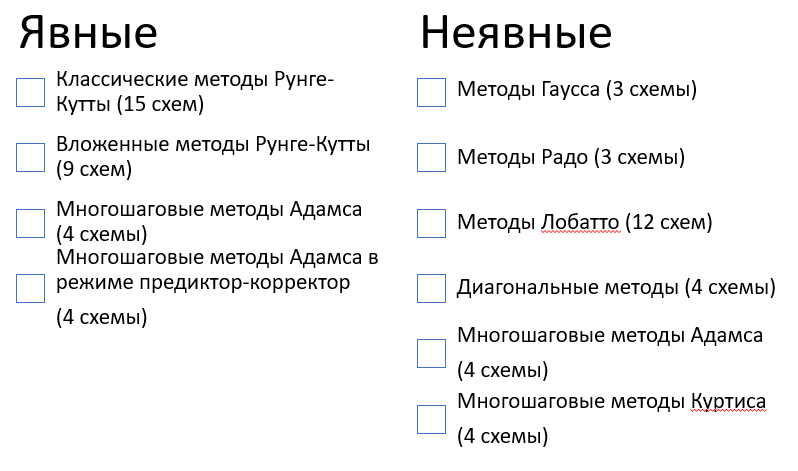
\includegraphics[width=15cm]{2-04-methods}
    \caption{Методы решения}
    \label{fig:SolveMethods}
\end{figure}

По желанию пользователя можно добавить другой метод при помощи специального конструктора.

\subsection{Схема Кранка-Николсона}

Для аппроксимации исходной системы уравнений \cite{book2} при моделировании течения спутных струй выбран неявный шеститочечный шаблон типа Кранка-Николсона с весами. На рисунке \ref{fig:crank} демонстрируется проблема использования чисто явной или чисто неявной схемы. Решение полученной системы нелинейных алгебраических уравнений определяется методом Гаусса.

\begin{figure}
    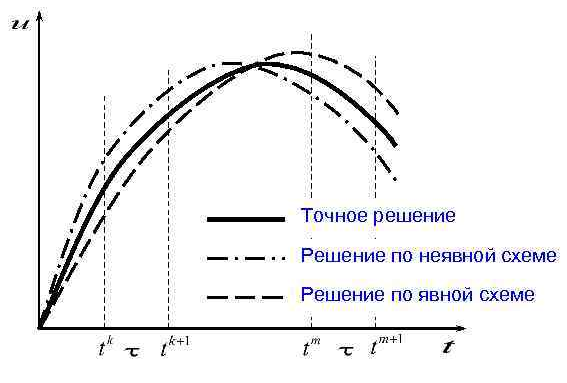
\includegraphics[width=10cm]{2-04-crank}
    \caption{Неявно-явные схемы с весами. Схема Кранка-Николсона}
    \label{fig:crank}
\end{figure}

К методам численного интегрирования уравнений обычно предъявляется ряд требований, выполнение которых желательно для создания эффективных программ расчета параметров течения. Это — сочетание скорости счета с достаточной точностью, применение сквозного метода без выделения характерных особенностей в разных зонах течения на основе устойчивой разностной схемы, и, наконец, универсальность по отношению к разным типам течений. Перечисленными свойствами обладает маршевый метод интегрирования с применением неявной разностной схемы на шеститочечном шаблоне типа Кранка-Николсона с весами. Он обладает вторым порядком точности по поперечной координате и первым или вторым порядком, в зависимости от параметра численной схемы, по продольной координате и относится к наиболее часто применяемым методам для решения задач параболизованного типа.

Решение каждой итерации происходит по следующей схеме:

\begin{itemize}
    \item в качестве приближённого решения берётся предыдущий слой;
    \item для каждого параметра уравнений ($U, V, W, J, T, \rho, P, C_i, i = 1,...,N$) строится трёхдиагональная матрица вида
    \begin{equation}
        A^mf_{n + 1}^{m + 1} + B^mf_{n + 1}^{m} + C^mf_{n + 1}^{m - 1} = D^m
    \end{equation}
    по заданной системе уравнений;
    \item матрица-система решается методом Гаусса, решение записывается в следующий слой;
    \item для достижения устойчивости решения, данная процедура повторяется 5 раз.
\end{itemize}

\subsection{Ввод данных по профилю}

Для корректного моделирования струйных течений необходимо точное задание начальных профилей параметров потока на входе в расчетную область. В работе используется ступенчатый профиль.

Ввод данных происходит посредством чтения таблицы профильных величин из тестового файла и чтения нулевых значений для перевода из профильных величин в физические. Сами по себе профильные величины позволяют уменьшить вероятность возникновения ошибки при вычислении больших значений, а значит ~--- повысить стабильность схемы, что будет продемонстрировано в следующем разделе во время тестирования.

Стоит отметить, что данный приём используется для параболизованной системы уравнений. Для полной системы Навье-Стокса при прямом вычислении все переменные записываются сразу в физических величинах.

\begin{table}
    \caption{Таблица профильных величин}
    \begin{tabular}{|c|c|c|c|c|c|}
    \hline
     Y &  U &   V &  W &   T &  P \\
    \hline
    0.100 & 1.000 & 0.000 & 0.000 & 1.000 & 1.000 \\
    0.200 & 1.000 & 0.000 & 0.000 & 1.000 & 1.000 \\
    0.300 & 1.000 & 0.000 & 0.000 & 1.000 & 1.000 \\
    0.400 & 1.000 & 0.000 & 0.000 & 1.000 & 1.000 \\
    0.500 & 1.000 & 0.000 & 0.000 & 1.000 & 1.000 \\
    0.600 & 1.000 & 0.000 & 0.000 & 1.000 & 1.000 \\
    0.700 & 1.000 & 0.000 & 0.000 & 1.000 & 1.000 \\
    0.800 & 1.000 & 0.000 & 0.000 & 1.000 & 1.000 \\
    0.900 & 1.000 & 0.000 & 0.000 & 1.000 & 1.000 \\
    1.000 & 1.000 & 0.000 & 0.000 & 1.000 & 0.455 \\
    1.100 & 1.000 & 0.000 & 0.000 & 1.000 & 0.182 \\
    1.200 & 0.820 & 0.000 & 0.000 & 0.740 & 0.036 \\
    1.300 & 0.797 & 0.000 & 0.000 & 0.433 & 0.036 \\
    1.400 & 0.797 & 0.000 & 0.000 & 0.433 & 0.036 \\
    1.500 & 0.797 & 0.000 & 0.000 & 0.433 & 0.045 \\
    1.600 & 0.797 & 0.000 & 0.000 & 0.433 & 0.054 \\
    1.700 & 0.797 & 0.000 & 0.000 & 0.433 & 0.061 \\
    1.800 & 0.797 & 0.000 & 0.000 & 0.433 & 0.061 \\
    1.900 & 0.797 & 0.000 & 0.000 & 0.433 & 0.061 \\
    \hline
    \end{tabular}
    \label{tab:profile}
\end{table}

Для ввода концентраций химических компонент используется отдельная таблица с идентичным форматом.

\subsection{Турбулентность}

В данной работе реализованы 3 модели турбулентности.

Для замыкания параболизованной системы уравнений~(\ref{eq1:navie_parabol1}-\ref{eq1:navie_parabol8}) при описании характеристик сверхзвуковой неизобарической струи в [11] рекомендуется использовать модификацию формулы Прандтля при числах $Pr = Sc = 0,07$:

\begin{equation}
    \mu_{T}=0.014 \rho U_{0} \Delta y_{1 / 2}\left(\Delta U_{m}\right)^{n}\left[|1-m| \frac{\Delta y_{1 / 2}}{y^{*}}+\left(1+\frac{\Delta y_{1 / 2}}{y^{*}}\right)\right],
\end{equation}
где
\begin{equation}
\label{eq2:helper_funcs}
\normalspacing
\begin{gathered}
\Delta U_{m}=\frac{U_{m}-U_{\mathrm{H}}}{U_{0}-U_{\mathrm{H}}}, \\
n=0.5-0.3 \sqrt{\frac{m}{1-m}}, \\
m=\frac{U_{\mathrm{H}}}{U_{0}}, \\
\Delta y_{1 / 2}=\left.y\right|_{\Delta J=0.2}-\left.y\right|_{\Delta J=0.8}, \\
y^{*}=\left.y\right|_{\Delta J=0.5}, \\
\Delta \bar{U}=\frac{U-U_{\mathrm{H}}}{U_{0}-U_{\mathrm{H}}}.
\end{gathered}
\end{equation}

Типичным примером демонстрации распределения газодинамических параметров служит расчёт течения изобарической изотермической одиночной струи. Коэффициент турбулентной вязкости, как и при построении точного решения, следует определить по формуле Прандтля [84]:

\begin{equation}
    \mu_{T}=\rho l^2 |\frac{\partial U}{\partial y}|,
\end{equation}
где$l = 0.11y_a$, $y_a$ ~--- ширина слоя смешения.

Другой пример посвящен расчету характеристик дозвукового течения коаксиальных $(W = 0)$ турбулентных неизотермических струй. Исследование основных закономерностей процесса смешения таких струй выполнено в [1] на основе обработки экспериментальных данных.  Влияние турбулентной вязкости учитывалось по модели, предложенной в [2]:

\begin{equation}
    \mu_{T}=0.0135\rho U_m \sqrt{0.07 + \left(1 - \frac{U_b}{U_m}\right)^2y_{1/2}},
\end{equation}
где $U_b$ ~---  скорость на внешней границе слоя смешения, а $U_m$ ~--— скорость на внутренней границе слоя смешения, причем
\begin{equation}
    y_{1/2} = \frac{1}{2}(\rho_bU_b + \rho_mU_m)
\end{equation}

В дальнейшем, в работу можно добавить реализацию моделей $SST$ или $k-\epsilon$.
